\chapter{L\normalsize ECTURE 1}
\section{Householder Transformation}
In the $n$-dim vector space $\mathbb{C}^n$, vector $x$ has:
selected a vector $v$, such that specific entities of 
transformed vector $x'$ equal to $0$. 
It workers as, selected vector $h$ gives equation 
\[
    x - 2 \langle x, v\rangle v
    = 
    x - 2 v (v^* x) 
    = 
    \left[
        x - 2vv^*
    \right]
    x
\]
where Transformation matrix 
$\left[
    x - 2vv^*
\right]$ 
denoted with $H$, and $2$ stands for the reflection.
\begin{figure}[H]
    \centering
    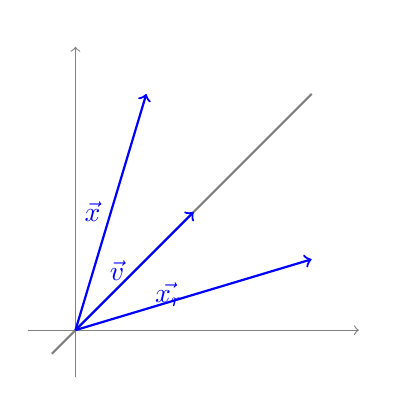
\begin{tikzpicture}[scale=3] % Adjust the scale as needed

        % Draw xOy plane
        \draw[gray, thin, ->] (-0.2,0) -- (1.2,0) node[anchor=north west] {};
        \draw[gray, thin, ->] (0,-0.2) -- (0,1.2) node[anchor=south east] {};
        
        \draw[gray, thick, .] (-0.1,-0.1) -- (1,1) node[midway, font=\small] {};
        % Draw the line from the origin to (0,0)
        \draw[blue, thick, ->] (0,0) -- (0.3,1) node[midway, anchor=east, font=\normalsize] {$\vec{x}$};
        \draw[blue, thick, ->] (0,0) -- (0.5,0.5) node[midway, anchor=east, font=\normalsize] {$\vec{v}$};
        \draw[blue, thick, ->] (0,0) -- (1,0.3) node[midway, anchor=east, font=\normalsize] {\red{$\vec{x_r}$}};
    \end{tikzpicture}
    \caption{Demonstration of Householder Transformation}
    \label{FIG1}
\end{figure} 
The $\vec{h}$ we discussed in lecture, is the orthogonal vector of $\vec{v}$ 
which follows 
\[
    \vec{h}
    = \pm 
    (\vec{x} - \vec{x_r}) 
\] 
and the sign is chosen for stability.
Most importantly, the $H$ has such propositions \ref{EQ:1}.
\begin{equation}\label{EQ:1}
    H = H^* = H^{-1}
\end{equation}
Thus, it gives us a shortcut 
for a sequential matrices series of $\left\{H_{k}\right\}_{k=1}^{n}$
which has 
\[
    \prod_{k=n}^{1}H_k A = R   
\] 
such that
\[
    A = 
    \prod_{k=1}^{n}H_k^{-1}
    R
    = \overbrace{ 
            \prod_{k=1}^{n}H_k^{*}
    }^{Q} 
    R
\]
